\documentclass[11pt,a4paper]{report}
\usepackage[textwidth=37em,vmargin=30mm]{geometry}
\usepackage{calc,xunicode,amsmath,amssymb,paralist,enumitem,tabu,booktabs,datetime2,xeCJK,xeCJKfntef,listings}
\usepackage{tocloft,fancyhdr,tcolorbox,xcolor,graphicx,eso-pic,xltxtra,xelatexemoji}

\newcommand{\envyear}[0]{2025}
\newcommand{\envdatestr}[0]{2025-07-31}
\newcommand{\envfinaldir}[0]{webdb/2025/20250731/final}

\usepackage[hidelinks]{hyperref}
\hypersetup{
    colorlinks=false,
    pdfpagemode=FullScreen,
    pdftitle={Web Digest - \envdatestr}
}

\setlength{\cftbeforechapskip}{10pt}
\renewcommand{\cftchapfont}{\rmfamily\bfseries\large\raggedright}
\setlength{\cftbeforesecskip}{2pt}
\renewcommand{\cftsecfont}{\sffamily\small\raggedright}

\setdefaultleftmargin{2em}{2em}{1em}{1em}{1em}{1em}

\usepackage{xeCJK,xeCJKfntef}
\xeCJKsetup{PunctStyle=plain,RubberPunctSkip=false,CJKglue=\strut\hskip 0pt plus 0.1em minus 0.05em,CJKecglue=\strut\hskip 0.22em plus 0.2em}
\XeTeXlinebreaklocale "zh"
\XeTeXlinebreakskip = 0pt


\setmainfont{Brygada 1918}
\setromanfont{Brygada 1918}
\setsansfont{IBM Plex Sans}
\setmonofont{JetBrains Mono NL}
\setCJKmainfont{Noto Serif CJK SC}
\setCJKromanfont{Noto Serif CJK SC}
\setCJKsansfont{Noto Sans CJK SC}
\setCJKmonofont{Noto Sans CJK SC}

\setlength{\parindent}{0pt}
\setlength{\parskip}{8pt}
\linespread{1.15}

\lstset{
	basicstyle=\ttfamily\footnotesize,
	numbersep=5pt,
	backgroundcolor=\color{black!5},
	showspaces=false,
	showstringspaces=false,
	showtabs=false,
	tabsize=2,
	captionpos=b,
	breaklines=true,
	breakatwhitespace=true,
	breakautoindent=true,
	linewidth=\textwidth
}






\newcommand{\coverpic}[2]{
    % argv: itemurl, authorname
    Cover photo by #2~~(\href{#1}{#1})
}
\newcommand{\makeheader}[0]{
    \begin{titlepage}
        % \newgeometry{hmargin=15mm,tmargin=21mm,bmargin=12mm}
        \begin{center}
            
            \rmfamily\scshape
            \fontspec{BaskervilleF}
            \fontspec{Old Standard}
            \fontsize{59pt}{70pt}\selectfont
            WEB\hfill DIGEST
            
            \vfill
            % \vskip 30pt
            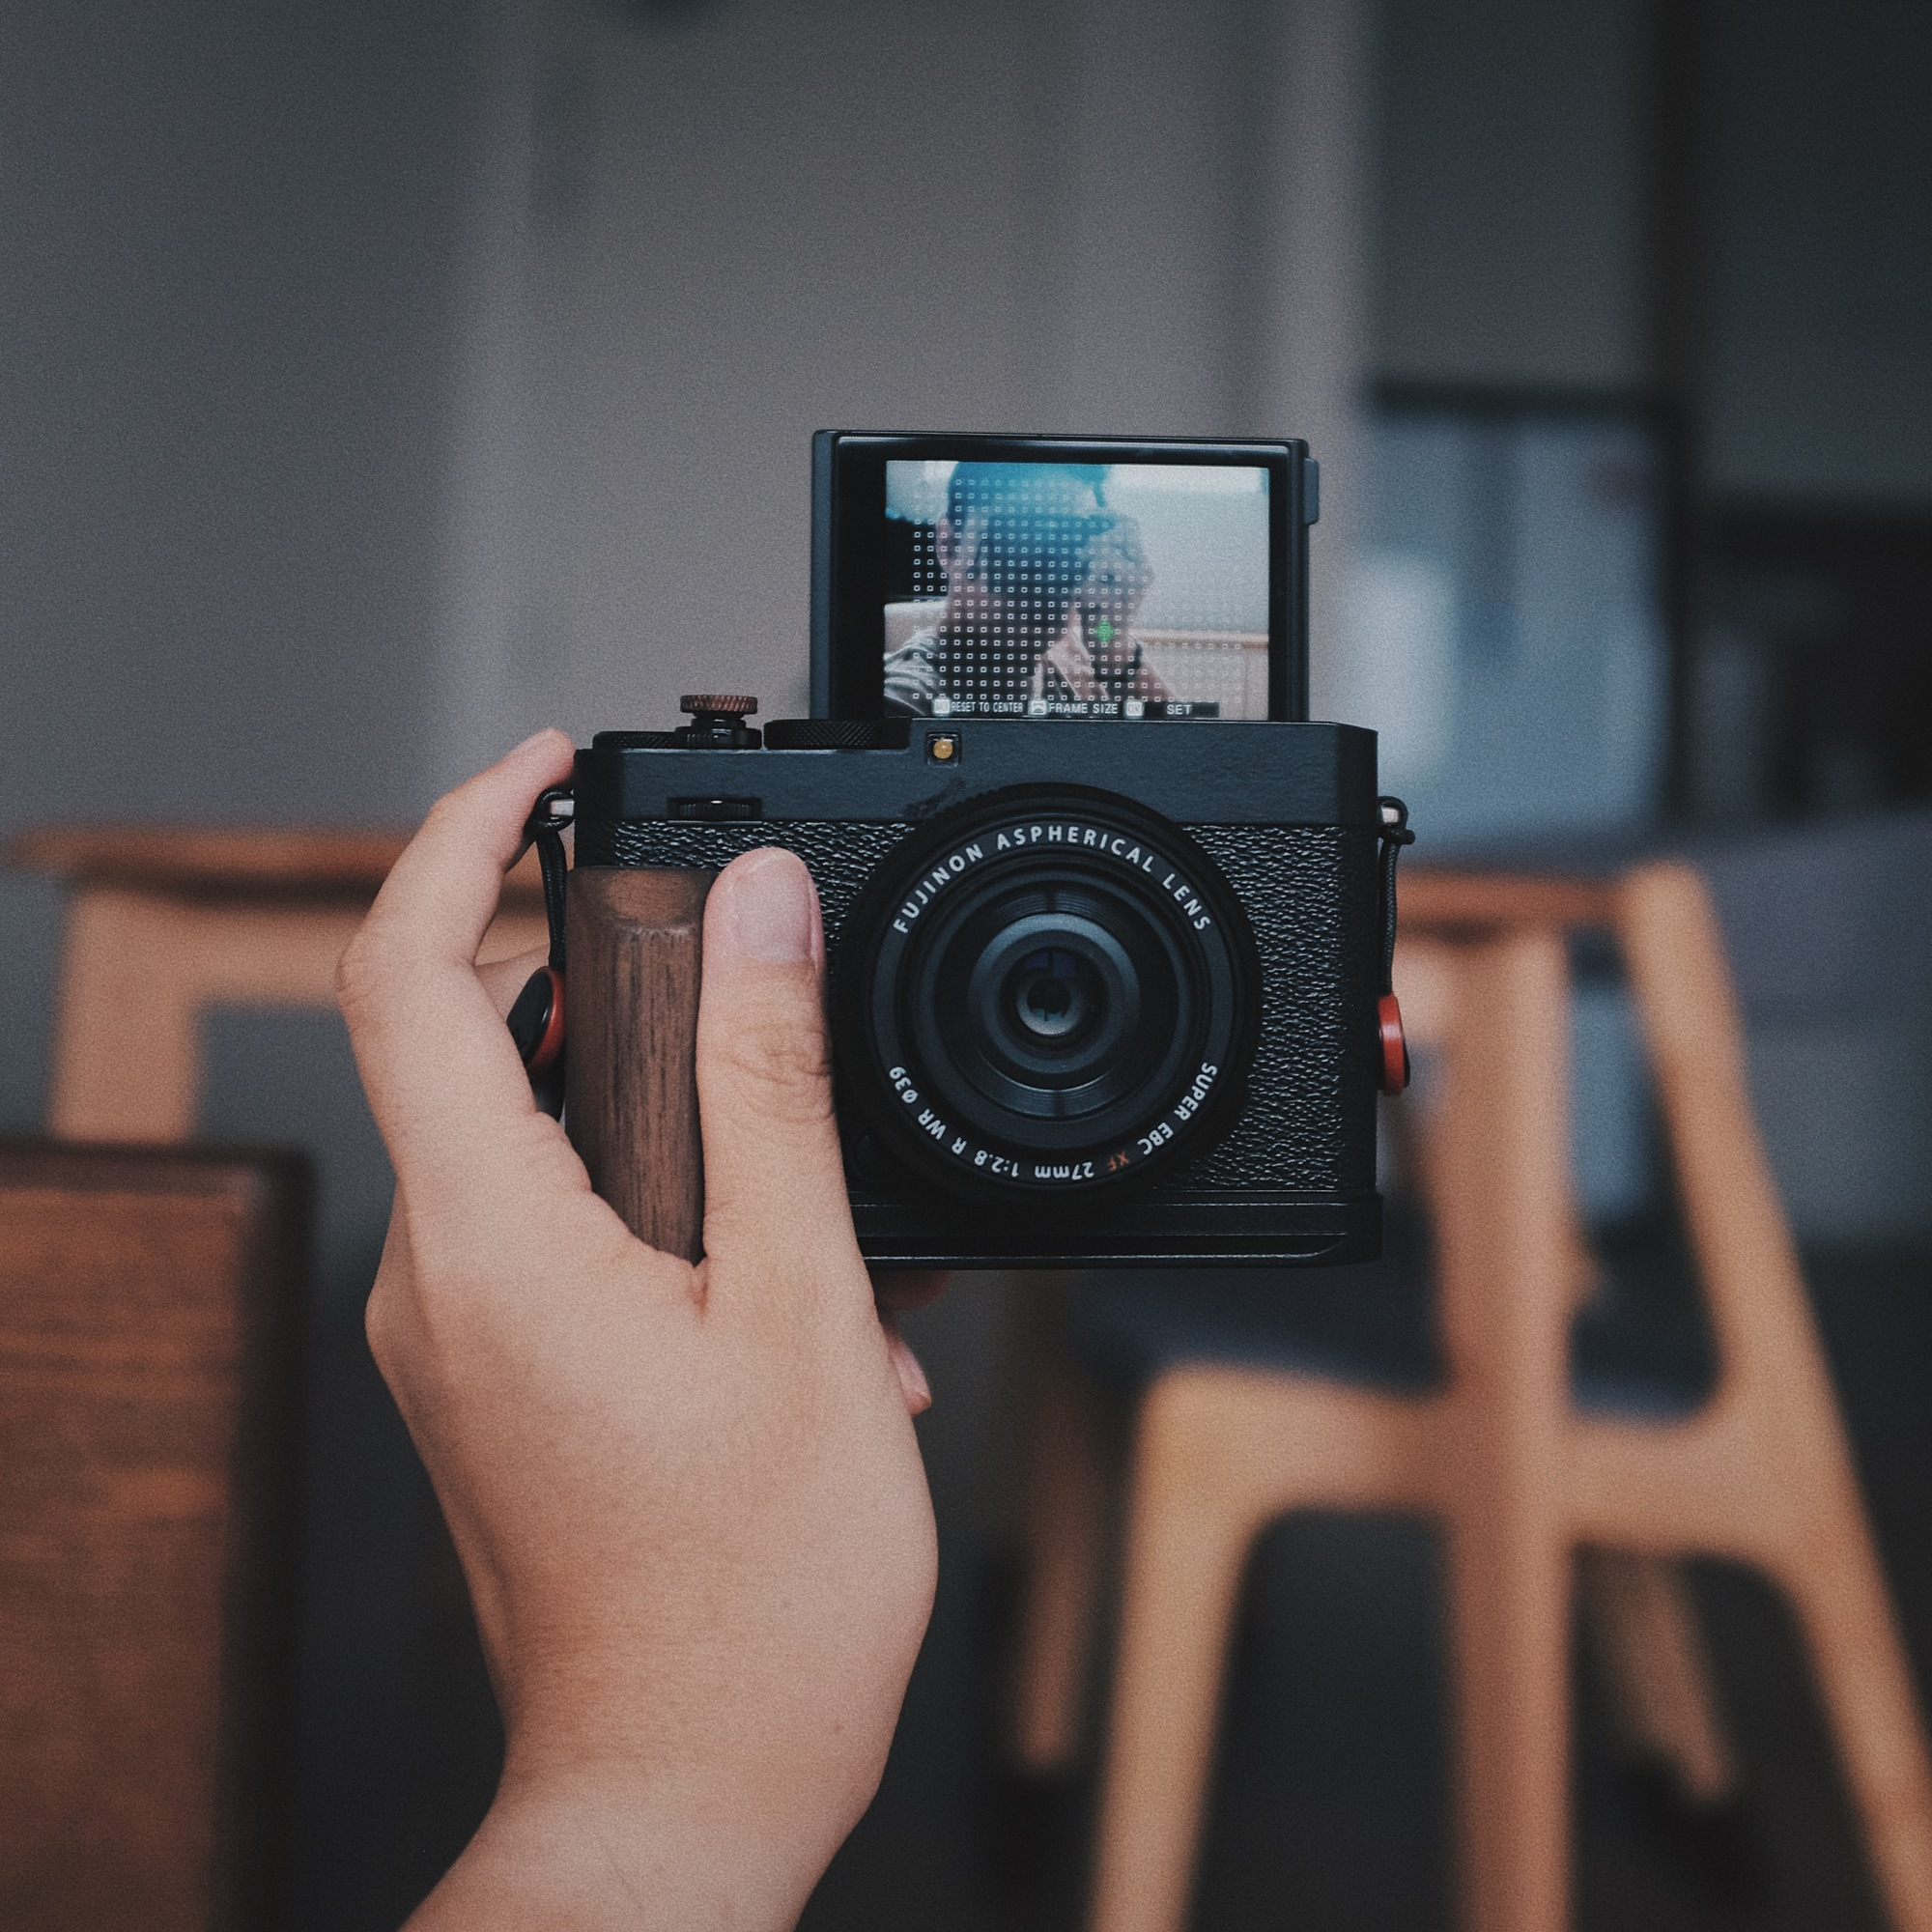
\includegraphics[width=\linewidth]{\envfinaldir/coverpic-prod.jpg}\par
            % \vskip 30pt
            \vfill

            \normalsize\rmfamily\scshape
            \copyright{} The Web Digest Project \hfill\large \envdatestr
        \end{center}
    \end{titlepage}
    % \restoregeometry
}
\newcommand{\simplehref}[1]{%
    \textcolor{blue!80!green}{\href{#1}{#1}}%
}
\renewcommand{\contentsname}{\center\Huge\sffamily\bfseries Contents\par\vskip 20pt}
\newcounter{ipartcounter}
\setcounter{ipartcounter}{0}
\newcommand{\ipart}[1]{
    % \vskip 20pt
    \clearpage
    \stepcounter{ipartcounter}
    \phantomsection
    \addcontentsline{toc}{chapter}{#1}
    % \begin{center}
    %     \Huge
    %     \sffamily\bfseries
    %     #1
    % \end{center}
    % \vskip 20pt plus 7pt
}
\newcounter{ichaptercounter}
\setcounter{ichaptercounter}{0}
\newcommand{\ichapter}[1]{
    % \vskip 20pt
    \clearpage
    \stepcounter{ichaptercounter}
    \phantomsection
    \addcontentsline{toc}{section}{\numberline{\arabic{ichaptercounter}}#1}
    \begin{center}
        \Huge
        \sffamily\bfseries
        #1
    \end{center}
    \vskip 20pt plus 7pt
}
\newcommand{\entrytitlefont}[1]{\subsection*{\raggedright\Large\sffamily\bfseries#1}}
\newcommand{\entryitemGeneric}[2]{
    % argv: title, url
    \parbox{\linewidth}{
        \entrytitlefont{#1}\par\vskip 5pt
        \footnotesize\ttfamily\mdseries
        \simplehref{#2}
    }\vskip 11pt plus 11pt minus 1pt
}
\newcommand{\entryitemGithub}[3]{
    % argv: title, url, desc
    \parbox{\linewidth}{
        \entrytitlefont{#1}\par\vskip 5pt
        \footnotesize\ttfamily\mdseries
        \simplehref{#2}\par\vskip 5pt
        \small\rmfamily\mdseries#3
    }\vskip 11pt plus 11pt minus 1pt
}
\newcommand{\entryitemAp}[3]{
    % argv: title, url, desc
    \parbox{\linewidth}{
        \entrytitlefont{#1}\par\vskip 5pt
        \footnotesize\ttfamily\mdseries
        \simplehref{#2}\par\vskip 5pt
        \small\rmfamily\mdseries#3
    }\vskip 11pt plus 11pt minus 1pt
}
\newcommand{\entryitemHackernews}[3]{
    % argv: title, hnurl, rawurl
    % \parbox{\linewidth}{
    %     \entrytitlefont{#1}\par\vskip 5pt
    %     \footnotesize\ttfamily\mdseries
    %     \simplehref{#3}\par
    %     \textcolor{black!50}{\href{#2}{#2}}
    % }\vskip 11pt plus 11pt minus 1pt
    \begin{minipage}{\linewidth}
            \entrytitlefont{#1}\par\vskip 5pt
            \footnotesize\ttfamily\mdseries
            \simplehref{#3}\par
            \textcolor{black!50}{\href{#2}{#2}}
    \end{minipage}\par\vskip 11pt plus 11pt minus 1pt
}







\begin{document}

\makeheader

\tableofcontents\clearpage




\ipart{Developers}
\ichapter{Hacker News}
\entryitemTwoLinks{Ollama has a native front end chatbot now}{https://news.ycombinator.com/item?id=44739632}{https://ollama.com/blog/new-app}

\entryitemTwoLinks{Vibe code is legacy code}{https://news.ycombinator.com/item?id=44739556}{https://blog.val.town/vibe-code}

\entryitemTwoLinks{Most Illinois farmland is not owned by farmers}{https://news.ycombinator.com/item?id=44737353}{https://www.chicagotribune.com/2025/06/01/illinois-farming-ownership-climate-change/}

\entryitemTwoLinks{The hype is the product}{https://news.ycombinator.com/item?id=44737346}{https://rys.io/en/180.html}

\entryitemTwoLinks{Fast}{https://news.ycombinator.com/item?id=44736967}{https://www.catherinejue.com/fast}

\entryitemTwoLinks{Australia widens teen social media ban to YouTube, scraps exemption}{https://news.ycombinator.com/item?id=44736646}{https://www.reuters.com/legal/litigation/australia-widens-teen-social-media-ban-youtube-scraps-exemption-2025-07-29/}

\entryitemTwoLinks{Crush: Glamourous AI coding agent for your favourite terminal}{https://news.ycombinator.com/item?id=44736176}{https://github.com/charmbracelet/crush}

\entryitemTwoLinks{Optician Sans – A free font based on historical eye charts and optotypes}{https://news.ycombinator.com/item?id=44736090}{https://optician-sans.com/}

\entryitemTwoLinks{Big Tech Killed the Golden Age of Programming}{https://news.ycombinator.com/item?id=44735081}{https://www.taylor.gl/blog/29}

\entryitemTwoLinks{Writing memory efficient C structs}{https://news.ycombinator.com/item?id=44733968}{https://tomscheers.github.io/2025/07/29/writing-memory-efficient-structs-post.html}

\entryitemTwoLinks{Try the Mosquito Bucket of Death}{https://news.ycombinator.com/item?id=44733888}{https://www.energyvanguard.com/blog/try-the-mosquito-bucket-of-death/}

\entryitemTwoLinks{Our \$100M Series B}{https://news.ycombinator.com/item?id=44733817}{https://oxide.computer/blog/our-100m-series-b}

\entryitemTwoLinks{I launched 17 side projects. Result? I'm rich in expired domains}{https://news.ycombinator.com/item?id=44733800}{https://news.ycombinator.com/item?id=44733800}

\entryitemTwoLinks{Problem solving often a matter of cooking up an appropriate Markov chain (2007)}{https://news.ycombinator.com/item?id=44733341}{http://math.uchicago.edu/~shmuel/Network-course-readings/Markov\_chain\_tricks.pdf}

\entryitemTwoLinks{The HTML Hobbyist}{https://news.ycombinator.com/item?id=44733119}{https://www.htmlhobbyist.com/}

\entryitemTwoLinks{Blog series on creating an OS in Rust}{https://news.ycombinator.com/item?id=44733094}{https://os.phil-opp.com/}

\entryitemTwoLinks{U.S. intelligence intervened with DOJ to push HPE-Juniper merger}{https://news.ycombinator.com/item?id=44732937}{https://www.axios.com/2025/07/30/merger-hpe-juniper-networks-national-security}

\entryitemTwoLinks{Sleep all comes down to the mitochondria}{https://news.ycombinator.com/item?id=44732020}{https://www.science.org/content/blog-post/it-all-comes-down-mitochondria}

\entryitemTwoLinks{`No Other Land' consultant Awdah Hathaleen killed by Israeli settler}{https://news.ycombinator.com/item?id=44731958}{https://www.latimes.com/entertainment-arts/story/2025-07-29/awdah-hathaleen-killed-no-other-land-palestinian-activist-israeli-settler}

\entryitemTwoLinks{M8.7 earthquake in Western Pacific, tsunami warning issued}{https://news.ycombinator.com/item?id=44729865}{https://earthquake.usgs.gov/earthquakes/eventpage/us6000qw60/executive}


\ipart{Developers~~~~(zh-Hans)}
\ichapter{Solidot}
\entryitemGeneric{\hskip 0pt{}Futurehome 申请破产后推送固件移除设备本地功能强推订阅制}{https://www.solidot.org/story?sid=81927}

\entryitemGeneric{\hskip 0pt{}微软承认它无法保障欧洲国家的数字主权}{https://www.solidot.org/story?sid=81926}

\entryitemGeneric{\hskip 0pt{}调查发现六成美国人将 AI 用于搜索 37\% 的人用于工作}{https://www.solidot.org/story?sid=81925}

\entryitemGeneric{\hskip 0pt{}印度对美智能手机出货量首次超过中国}{https://www.solidot.org/story?sid=81924}

\entryitemGeneric{\hskip 0pt{}Opera 指控微软使用反竞争策略推广自家浏览器 Edge }{https://www.solidot.org/story?sid=81923}

\entryitemGeneric{\hskip 0pt{}微软封禁 LibreOffice 开发者账号}{https://www.solidot.org/story?sid=81922}

\entryitemGeneric{\hskip 0pt{}俄罗斯堪察加半岛发生 M8.8 级地震}{https://www.solidot.org/story?sid=81921}

\entryitemGeneric{\hskip 0pt{}成人网站指控 Meta 下载和做种成人视频}{https://www.solidot.org/story?sid=81920}

\entryitemGeneric{\hskip 0pt{}经济学家称挪威人太富裕且太舒坦了}{https://www.solidot.org/story?sid=81919}

\entryitemGeneric{\hskip 0pt{}中国大学鼓励学生使用 AI}{https://www.solidot.org/story?sid=81918}

\entryitemGeneric{\hskip 0pt{}未成年人参与了秦兵马俑的制作}{https://www.solidot.org/story?sid=81917}

\entryitemGeneric{\hskip 0pt{}北京火狐从 9 月 29 日起不再运营 Firefox 在华业务}{https://www.solidot.org/story?sid=81916}

\entryitemGeneric{\hskip 0pt{}银河系发现首个幽灵行星状星云}{https://www.solidot.org/story?sid=81915}

\entryitemGeneric{\hskip 0pt{}教育能否延缓认知衰退?}{https://www.solidot.org/story?sid=81914}

\entryitemGeneric{\hskip 0pt{}安全研究员发现 SkyRover X1 是更换品牌的大疆产品}{https://www.solidot.org/story?sid=81913}

\entryitemGeneric{\hskip 0pt{}人类组织蛋白质在 50 岁左右加速衰老}{https://www.solidot.org/story?sid=81912}

\entryitemGeneric{\hskip 0pt{}三星 One UI 8 禁止解锁 bootloader}{https://www.solidot.org/story?sid=81911}

\entryitemGeneric{\hskip 0pt{}索尼指控腾讯抄袭其《地平线》系列游戏}{https://www.solidot.org/story?sid=81910}

\entryitemGeneric{\hskip 0pt{}在 Online Safety Act 生效后英国 VPN 使用量激增}{https://www.solidot.org/story?sid=81909}

\entryitemGeneric{\hskip 0pt{}挪威开始在海底储存液化二氧化碳}{https://www.solidot.org/story?sid=81908}\ichapter{V2EX}
\entryitemGeneric{\hskip 0pt{}[酷工作] [Lime][2025] 招聘资深后端工程师,全职远程岗}{https://www.v2ex.com/t/1148898}

\entryitemGeneric{\hskip 0pt{}[问与答] Google 帮我备份的短信和通话记录怎么查询或恢复到新手机?}{https://www.v2ex.com/t/1148897}

\entryitemGeneric{\hskip 0pt{}[问与答] 自建云平台方案}{https://www.v2ex.com/t/1148896}

\entryitemGeneric{\hskip 0pt{}[Apple] 更新 Sequoia 到 macOS 15.6, 好像能解决本地网络权限下, 有多个 Chrome 条目的问题}{https://www.v2ex.com/t/1148895}

\entryitemGeneric{\hskip 0pt{}[程序员] 感觉这两年 PostgreSQL 明显越来越火了}{https://www.v2ex.com/t/1148894}

\entryitemGeneric{\hskip 0pt{}[iCloud] Mac 上同步到 iCloud 的 Excel 文件,在 iPhone 上打开后居然直接使用旧版本覆盖了新版本}{https://www.v2ex.com/t/1148892}

\entryitemGeneric{\hskip 0pt{}[宽带症候群] 跨网 boom 时代下骨干网大手所映射出的问题}{https://www.v2ex.com/t/1148891}

\entryitemGeneric{\hskip 0pt{}[电动汽车] 2025 年 7 月开特斯拉游加拿大海洋三省的充电情况和自动驾驶使用体验}{https://www.v2ex.com/t/1148890}

\entryitemGeneric{\hskip 0pt{}[酷工作] Plaud AI 招聘啦!}{https://www.v2ex.com/t/1148888}

\entryitemGeneric{\hskip 0pt{}[职场话题] V 友们,搬砖副业求指导}{https://www.v2ex.com/t/1148887}

\entryitemGeneric{\hskip 0pt{}[全球工单系统] 小龙,为什么你不让我叫 Emoji 名字了? \#微信}{https://www.v2ex.com/t/1148886}

\entryitemGeneric{\hskip 0pt{}[酷工作] [兼职远程] UI 设计师}{https://www.v2ex.com/t/1148885}

\entryitemGeneric{\hskip 0pt{}[问与答] 阿里小号即将下线,用什么替代?}{https://www.v2ex.com/t/1148884}

\entryitemGeneric{\hskip 0pt{}[程序员] 字节的 SeedEdit 图像编辑模型今天发布了,应该是目前最强的修图大模型了}{https://www.v2ex.com/t/1148883}

\entryitemGeneric{\hskip 0pt{}[问与答] github 的 project 的最佳实践是什么?}{https://www.v2ex.com/t/1148882}

\entryitemGeneric{\hskip 0pt{}[Solana] 打赏为啥提示:发起交易失败: Unexpected error}{https://www.v2ex.com/t/1148880}

\entryitemGeneric{\hskip 0pt{}[职场话题] 入行两年有点迷茫了,想请教前辈们是如何找到持续精进方向的?}{https://www.v2ex.com/t/1148879}

\entryitemGeneric{\hskip 0pt{}[程序员] 最纯粹的开源接口开发测试工具发布 v0.0.20}{https://www.v2ex.com/t/1148878}

\entryitemGeneric{\hskip 0pt{}[数据库] [新手求建议] 结构化数据,波形图为主,用于识别模型训练有没有推荐的数据库?}{https://www.v2ex.com/t/1148877}

\entryitemGeneric{\hskip 0pt{}[macOS] AlDente 发布了 beta 版 1.33.2 支持 macOS Tahoe 26, 测试有效}{https://www.v2ex.com/t/1148876}

\entryitemGeneric{\hskip 0pt{}[Android] 原装安卓系统用浏览器看视频的时候,调用的播放器可以换成其他的么?}{https://www.v2ex.com/t/1148875}

\entryitemGeneric{\hskip 0pt{}[生活] 大学网友近 1W+的欠款 近 10 年今天终于联系上了,也很顺利的还了}{https://www.v2ex.com/t/1148874}

\entryitemGeneric{\hskip 0pt{}[API] PPT 转高精度图片 API 接口}{https://www.v2ex.com/t/1148872}

\entryitemGeneric{\hskip 0pt{}[Solana] 作为之前从来没有过虚拟货币经验的小白,和大家分享一下如何购买 SOL、V2EX 代币超简单流程}{https://www.v2ex.com/t/1148870}

\entryitemGeneric{\hskip 0pt{}[问与答] 杭州地区有用移动互联网专线作为公司宽带使用的吗?}{https://www.v2ex.com/t/1148869}

\entryitemGeneric{\hskip 0pt{}[OpenAI] 分享一下 ChatGPT Study Mode System Prompt}{https://www.v2ex.com/t/1148867}

\entryitemGeneric{\hskip 0pt{}[宽带症候群] 如果肉身翻不了墙,就隐居去}{https://www.v2ex.com/t/1148866}

\entryitemGeneric{\hskip 0pt{}[MacBook] 智障吗? macbook 居然不能关机或按键开机}{https://www.v2ex.com/t/1148864}

\entryitemGeneric{\hskip 0pt{}[Apple] Apple Watch 户外跑步疑问}{https://www.v2ex.com/t/1148863}

\entryitemGeneric{\hskip 0pt{}[分享创造] GeminiCLI 转 API 服务, Kiro 转 API 服务,免费使用 Gemini 和 Claude 大模型}{https://www.v2ex.com/t/1148862}

\entryitemGeneric{\hskip 0pt{}[酷工作] 帮朋友公司发布两个招聘需求,坐标杭州,一个前端一个后端。}{https://www.v2ex.com/t/1148861}

\entryitemGeneric{\hskip 0pt{}[问与答] 帕米康的随身 wifi 怎么样,续费¥ 14.8 300g 流量}{https://www.v2ex.com/t/1148860}

\entryitemGeneric{\hskip 0pt{}[Nintendo Switch] 任天堂家庭会员上车}{https://www.v2ex.com/t/1148859}

\entryitemGeneric{\hskip 0pt{}[NAS] 请教是不是可以设置 ha.com 然后劫持并访问我的 192.168.31.3:8123 的 homeassistant 地址?}{https://www.v2ex.com/t/1148858}

\entryitemGeneric{\hskip 0pt{}[职场话题] 毕业}{https://www.v2ex.com/t/1148857}

\entryitemGeneric{\hskip 0pt{}[分享创造] Vibe coding 了一个 V2EX.meme \$V2EX 价格实时查询}{https://www.v2ex.com/t/1148856}

\entryitemGeneric{\hskip 0pt{}[汽车] 猛士 817 不错}{https://www.v2ex.com/t/1148855}

\entryitemGeneric{\hskip 0pt{}[iPhone] 有没有办法阻止 iPhone 强制重启验证登录呢}{https://www.v2ex.com/t/1148854}

\entryitemGeneric{\hskip 0pt{}[以太坊] 我从币安提现 eth,为啥钱包 account 1 的 eth 地址只可以用 BSC 网络, account 2 的地址却 BSC 和 ETH 网络都可以用?}{https://www.v2ex.com/t/1148853}

\entryitemGeneric{\hskip 0pt{}[奇思妙想] 有没有人对最近的奥默默 2 号感兴趣}{https://www.v2ex.com/t/1148851}

\entryitemGeneric{\hskip 0pt{}[酷工作] [招聘|远程] 百万年薪|硅谷 stealth 初创招聘爬虫大佬}{https://www.v2ex.com/t/1148850}

\entryitemGeneric{\hskip 0pt{}[投资] 有没有投资美股港股被要求补税的大佬}{https://www.v2ex.com/t/1148849}

\entryitemGeneric{\hskip 0pt{}[路由器] 大佬们,求推荐 wifi7 路由器 mesh 方案}{https://www.v2ex.com/t/1148848}

\entryitemGeneric{\hskip 0pt{}[分享发现] 一款在浏览器中运行的录音机}{https://www.v2ex.com/t/1148847}

\entryitemGeneric{\hskip 0pt{}[问与答] 怎么跟空降领导相处比较好}{https://www.v2ex.com/t/1148845}

\entryitemGeneric{\hskip 0pt{}[分享发现] AI 交流群,欢迎加入👏}{https://www.v2ex.com/t/1148844}

\entryitemGeneric{\hskip 0pt{}[浏览器] 如何导出、永久保存浏览器历史记录? [风无前]}{https://www.v2ex.com/t/1148843}

\entryitemGeneric{\hskip 0pt{}[问与答] , macOS sonoma 如何关闭的窗口缩小与打开动画效果?}{https://www.v2ex.com/t/1148842}

\entryitemGeneric{\hskip 0pt{}[问与答] 都说微信输入法好用,通讯录人名输入怎么解决?}{https://www.v2ex.com/t/1148841}

\entryitemGeneric{\hskip 0pt{}[问与答] 现在比较有性价比的长期 GPU 租赁推荐哪些平台?}{https://www.v2ex.com/t/1148840}


\ipart{Generic News}







\clearpage
\leavevmode\vfill
\footnotesize

Copyright \copyright{} 2023-2025 Neruthes and other contributors.

This document is published with CC BY-NC-ND 4.0 license.

The entries listed in this newsletter may be copyrighted by their respective creators.

This newsletter is generated by the Web Digest project.

The newsletters are also delivered via Telegram channel \CJKunderline{\href{https://t.me/webdigestchannel}{https://t.me/webdigestchannel}}.\\
RSS feed is available at \CJKunderline{\href{https://webdigest.pages.dev/rss.xml}{https://webdigest.pages.dev/rss.xml}}.

This newsletter is available in PDF at
\CJKunderline{\href{https://webdigest.pages.dev/}{https://webdigest.pages.dev/}}.

The source code being used to generate this newsletter is available at\\
\CJKunderline{\href{https://github.com/neruthes/webdigest}{https://github.com/neruthes/webdigest}}.

This newsletter is also available in
\CJKunderline{\href{http://webdigest.pages.dev/readhtml/\envyear/WebDigest-20250731.html}{HTML}} and
\CJKunderline{\href{https://github.com/neruthes/webdigest/blob/master/markdown/\envyear/WebDigest-20250731.md}{Markdown}}.


\coverpic{https://unsplash.com/photos/blue-jellyfish-floating-in-the-black-abyss-NDQbSIBQEi0}{Mykhailo Amirdzhanian}


\end{document}
